% \chapter{Multimodal Systems}

% \section{Multimodality}
% To develop our multimodal system we will start with a very simple model with the assumption that the applied $\vec{B}$ field is parallel to the defect axis. From there we will iterate our ensemble and work to reduce the number of assumptions.
%

\section{Proposed Systems}
We have described schemas for measuring the $\vec{E}$ field, $\vec{B}$ field, temperature, pressure and strain. We will say that the measurement of $T$ and $P$ should be considered equivalent in a $S=1$ system and the measurement of strain is equivalent to $\vec{E}$ in all systems.

Thus, we have $^4 C _2 = 6$ distinct pairwise combinations we may consider for multimodal application:
($\vec{B}$, $T$), ($\vec{B}$, $P$), ($\vec{B}$, $\vec{E}$), ($\vec{E}$, $T$), ($\vec{E}$, $P$) and ($T$, $P$).

We will discuss the combinations for which multi-modality is possible using the techniques described in this work.
% If not possible, we discuss why and if development of the literature could make such a sensor possible. 
Throughout the discussion, all external parameters not discussed are assumed to be absent.

% \subsection{$\vec{B}$ Multimode}
\subsection{$\vec{B}$ and Temperature}\label{sec:multimode_BT}
In general, simultaneously measuring $\vec{B}$ and $T$ is not possible as when the magnetic field is at $\theta \neq 90$, ZFS $D$ may not be inferred from the ODMR spectra. However, aligning $\vec{B}$ perpendicular to the defect axis allows $D$ to be calculated from the spectra and the magnitude of the field to be measured. 

\begin{proposal}{$|\vec{B}|$ and Temperature}
	We exploit the temperature independence of the V2 Silicon vacancy to measure the $\vec{B}$ field. Temperature may then be measured by either the same defect using anti-Stokes technique or a divacancy where temperature may be inferred from the change in ZFS $D$.
\end{proposal}
\begin{figure}[h]
	\begin{center}
		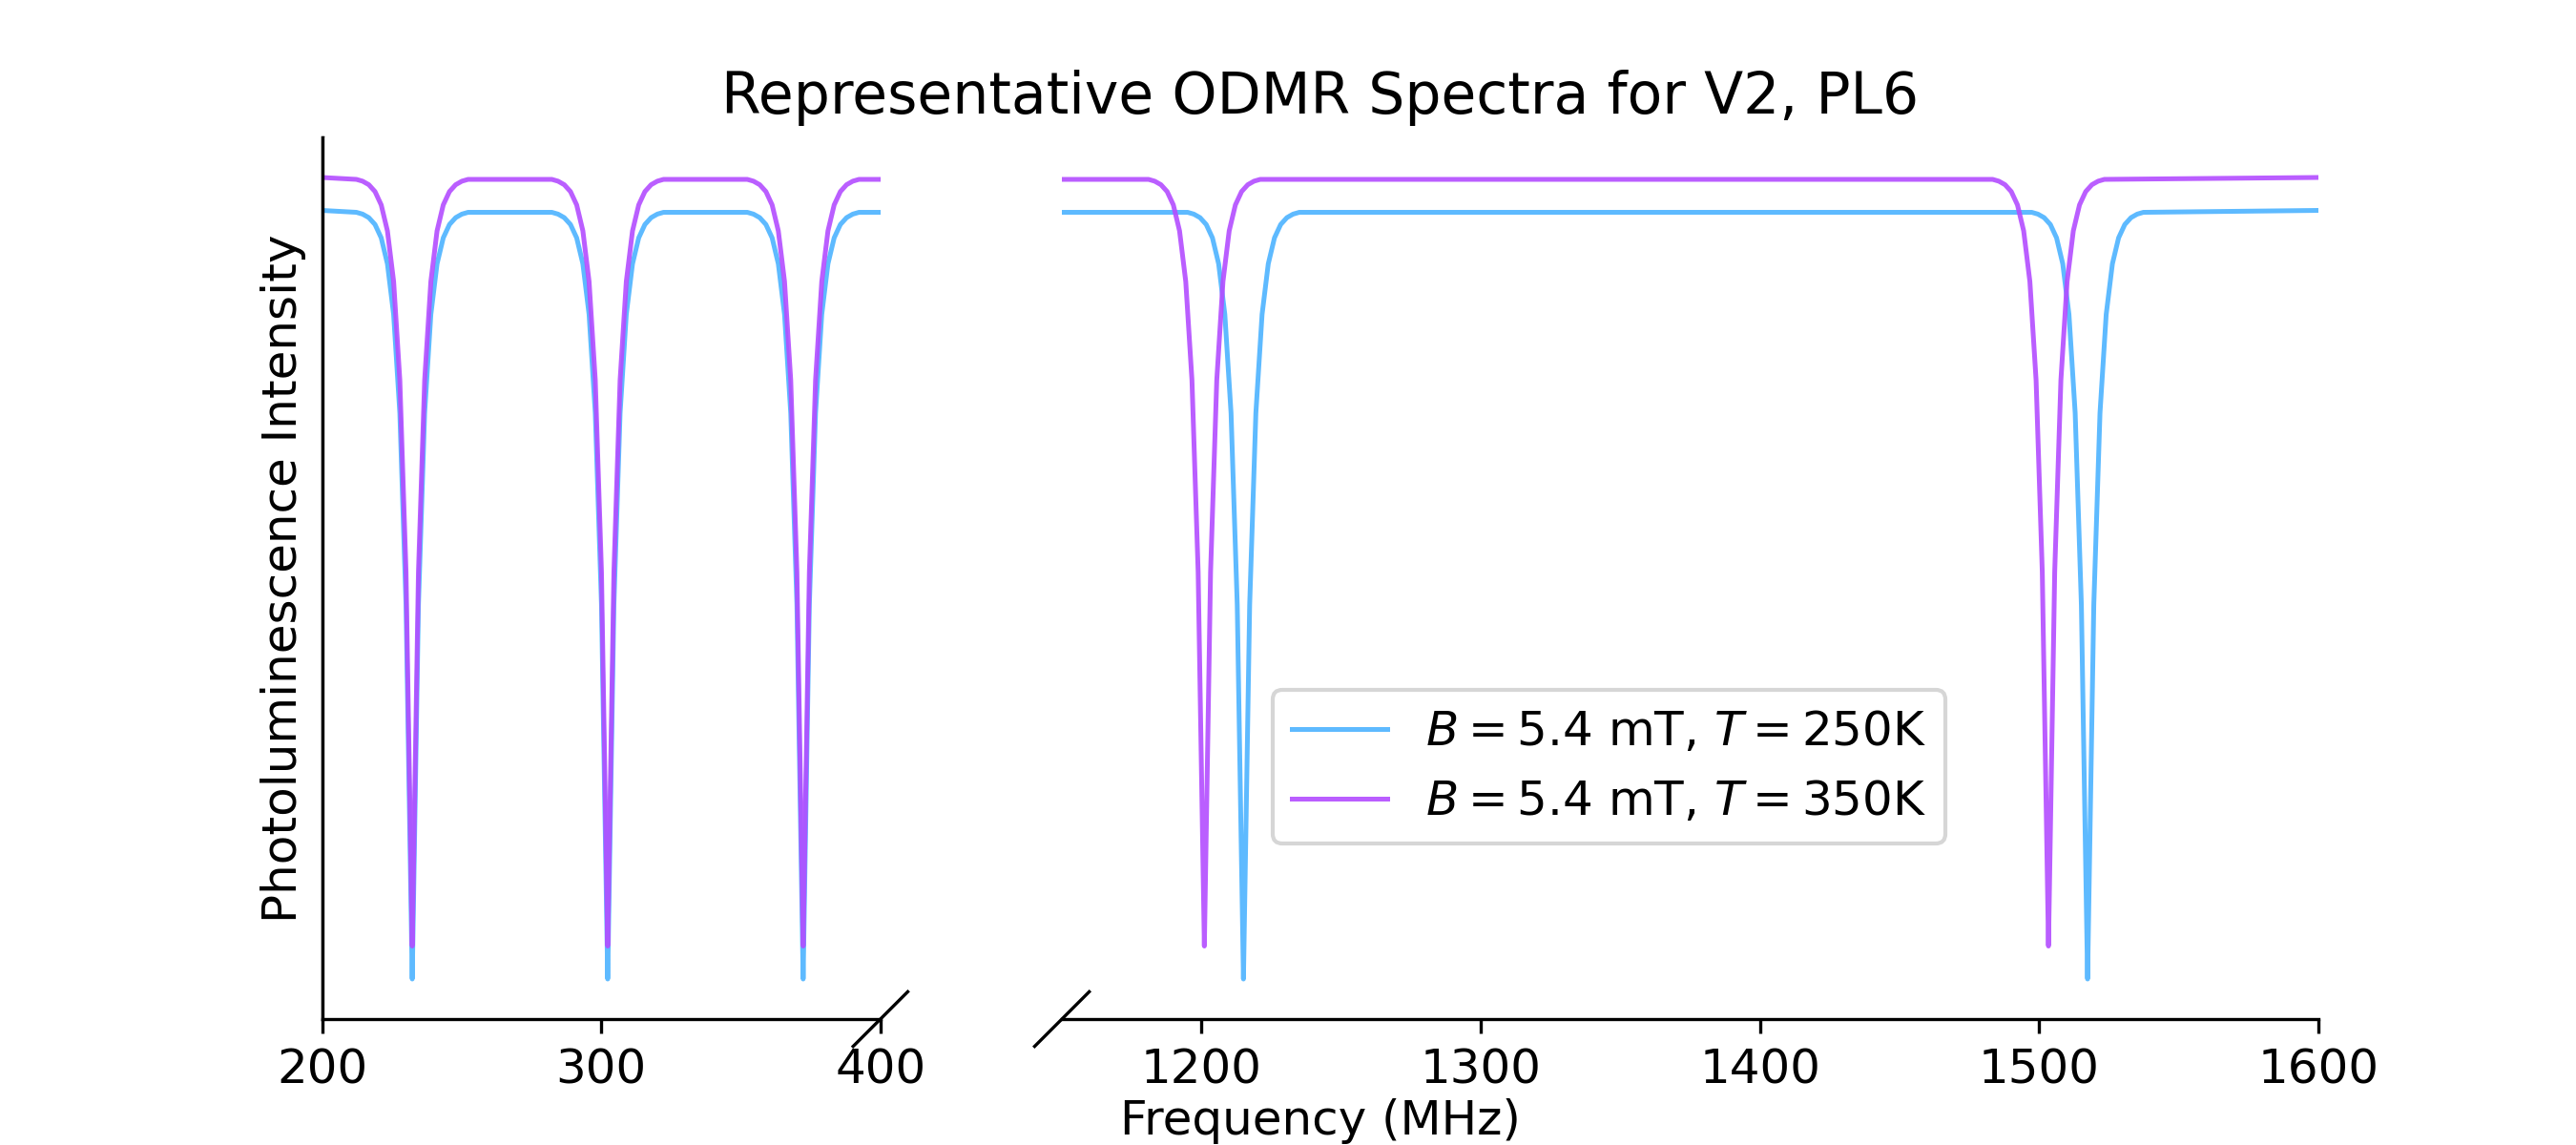
\includegraphics[width=0.95\textwidth]{figures/ODMR-multimodal-s15magnet-s1T.png}
	\end{center}
	\caption{}\label{fig:multimode_BT}
    \todo[inline, color=ediblue]{Write caption}
\end{figure}
The implementation is to capture the ODMR spectra of the defects. Figure \ref{fig:multimode_BT} shows a two simulated spectra for a V2 and PL6 ensemble at 250K and 350K (offset for clarity). Clearly the V2 spectra is unaffected by temperature allowing $\vec{B}$ to be measured from the three frequencies as described in summary \ref{sum:spin1.5magnet}. Providing the ZFS $D$ of the PL6 is under no other influence e.g. pressure or $\vec{E}_\parallel$, $D(T)$ may be read from the two frequencies of the PL6 defect as described in \ref{sum:spin1thermo}.





\subsection{$\vec{B}$ and Pressure}
As for \ref{sec:multimode_BT} this is not possible in general and required $\vec{B}$ to be perpendicular to the defect axis. 

\begin{proposal}{$|\vec{B}$| and Pressure}
	We exploit the linear dependence of the V2 Silicon vacancy $D$ and pressure, and the linear dependence on $\Delta f$ of the divacancy on the applied $\vec{B}$ field. We determine the pressure from the average of the two EPR frequencies for the divacancy and use the inferred pressure to perform magnetometry. 

\end{proposal}

\begin{figure}[h]
	\begin{center}
		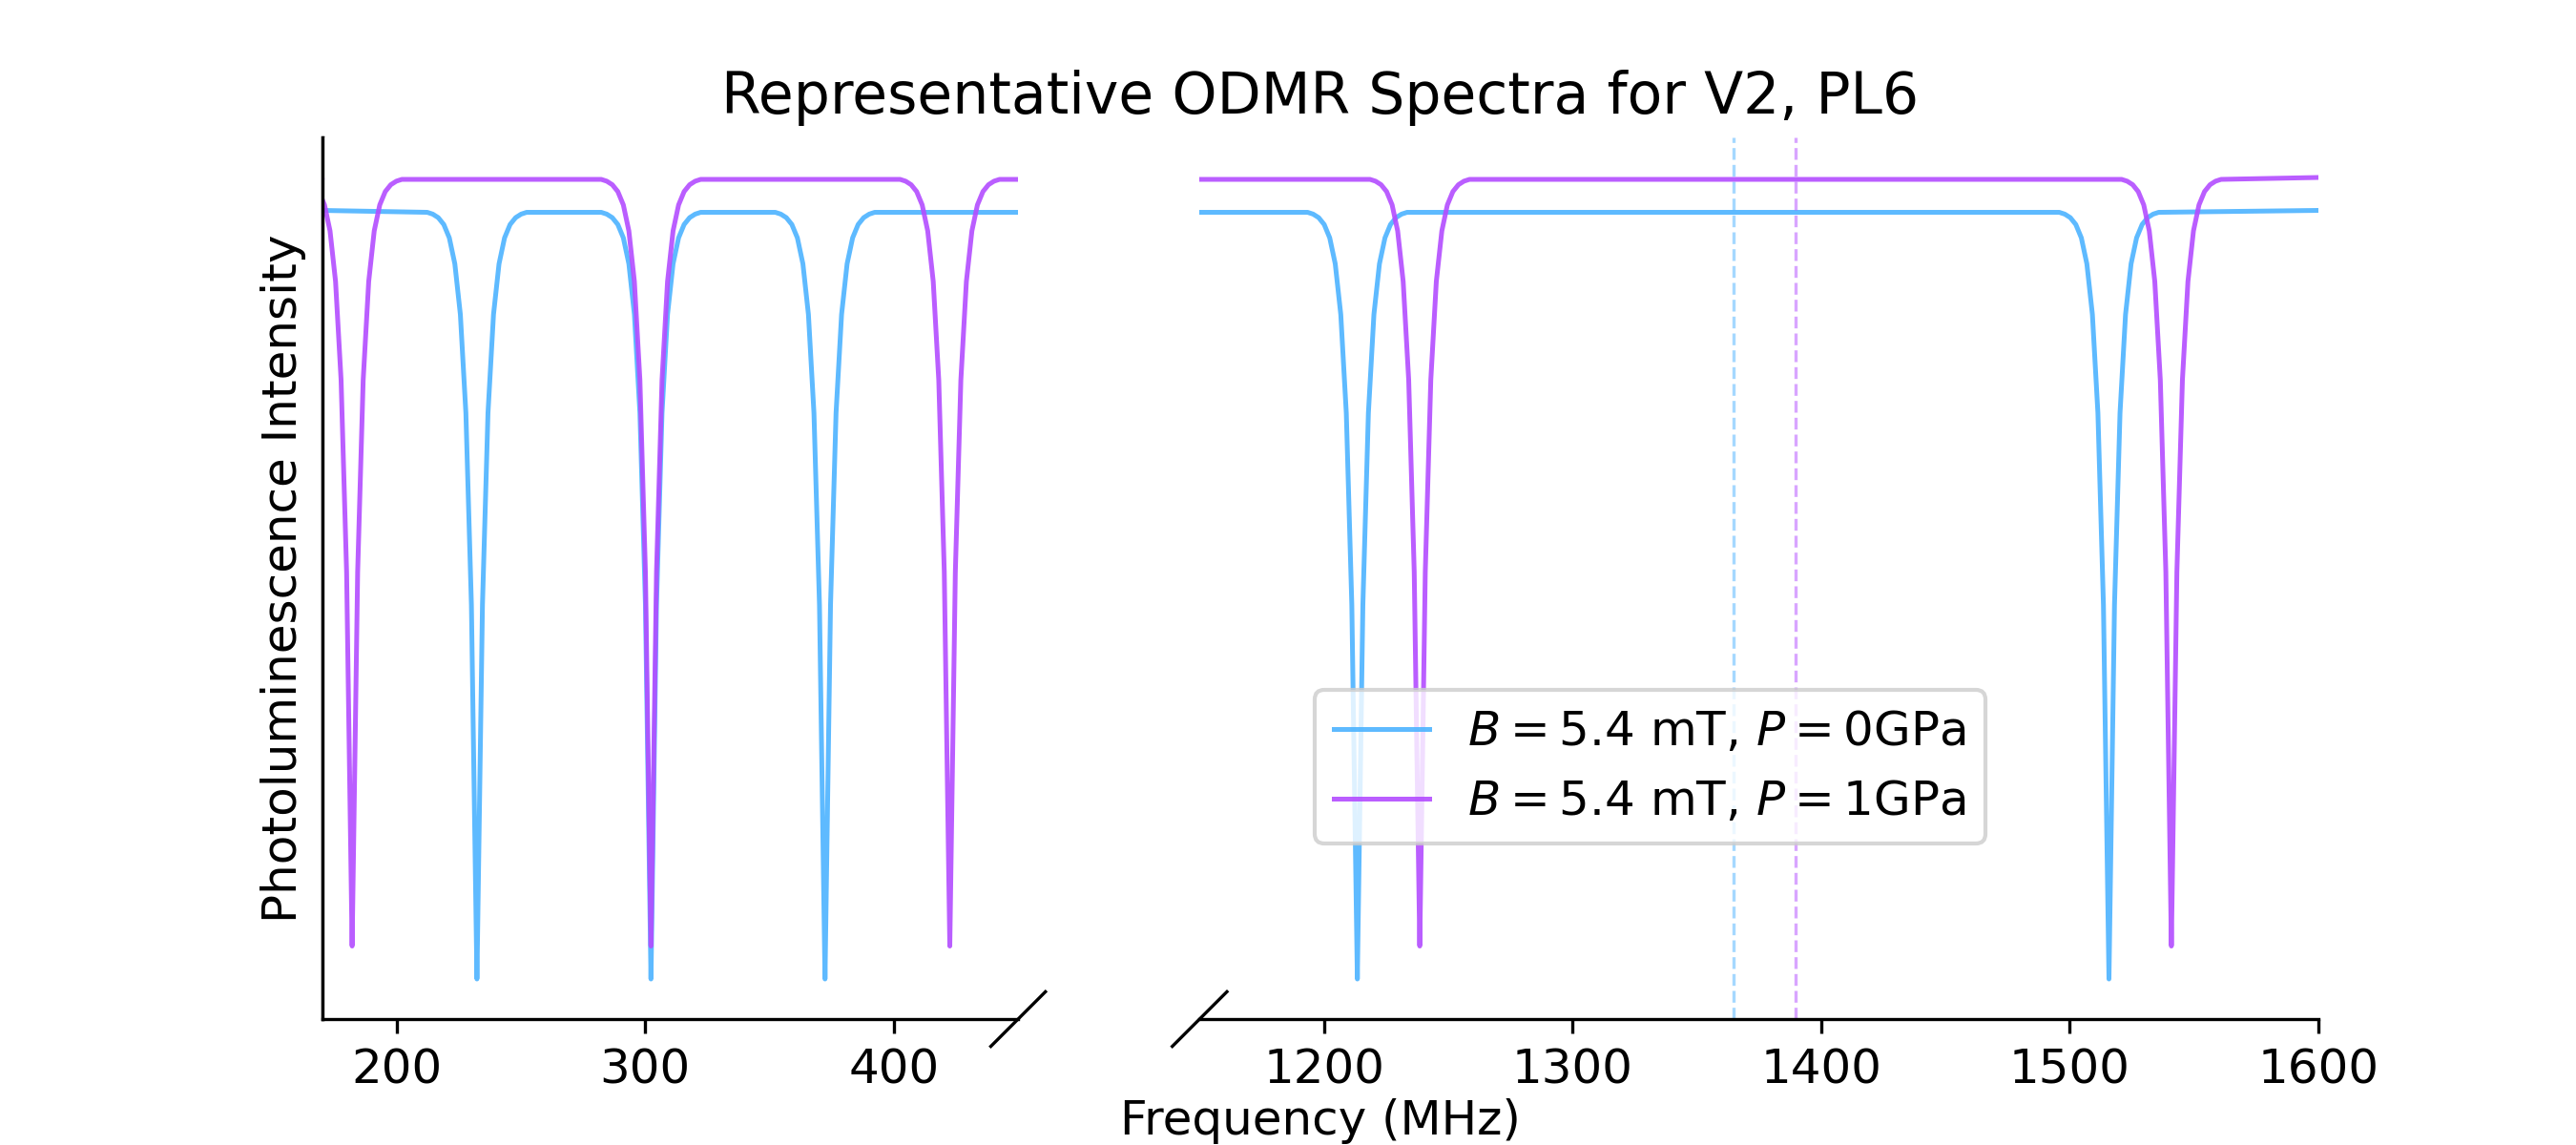
\includegraphics[width=0.95\textwidth]{figures/ODMR-multimodal-s15magnet-s1P.png}
	\end{center}
	\caption{}\label{fig:multimode_BP}
    \todo[inline, color=ediblue]{Write caption}
\end{figure}

The approach is slightly less straight forward as the ZFS $D$ of the Silicon vacancy shows a linear dependence on $P$. Thus, we cannot cleanly separate the two parameters as above. However, since the dependence is linear, as is the dependence of an $S=1$ defect splitting on the $\vec{B}$ field, and the $B$ field does not influence $D$, we may still determine the parameters simultaneously.

The implementation is to first measure $D(P)$ by taking the average of the two frequencies of the $S=1$ defect (\ref{sum:spin1.5thermo}). Now the pressure is known, calculate $D(P)$ for the Silicon vacancy and perform magnetometry with the V2 Silicon vacancy as detailed in \ref{sum:spin1.5magnet}.


\subsection{Temperature and Pressure}\label{multi_TP}
Simultaneously measuring temperature and pressure
% is not currently possible due to a lack of understanding of the interplay between $T$ and $P$ and the combined effect on $D$.
may be achieved using only the V2 Silicon vacancy. Illustrative ODMR plots are shown with $\vec{B}$ applied parallel to the defect axis. 

\begin{proposal}{Temperature and Pressure}
    The temperature independence of the V2 Silicon vacancy allows the CW-ODMR spectra to be inspected to evaluate $P$ from $D(P)$. 
    With knowledge of the effective $D$, tune two lasers to a Stokes and anti-Stokes frequency and perform $S=3/2$ temperature measurements. 
\end{proposal}


The ODMR spectra of the V2 Silicon vacancy in zero field (magnetic or electric) will show a single peak at the effective $D$. 
This may be used to determine the position of the zero phonon line from which temperature measurement can be performed as described in \ref{sum:spin1.5thermo}. 

\begin{figure}[h]
    \begin{center}
        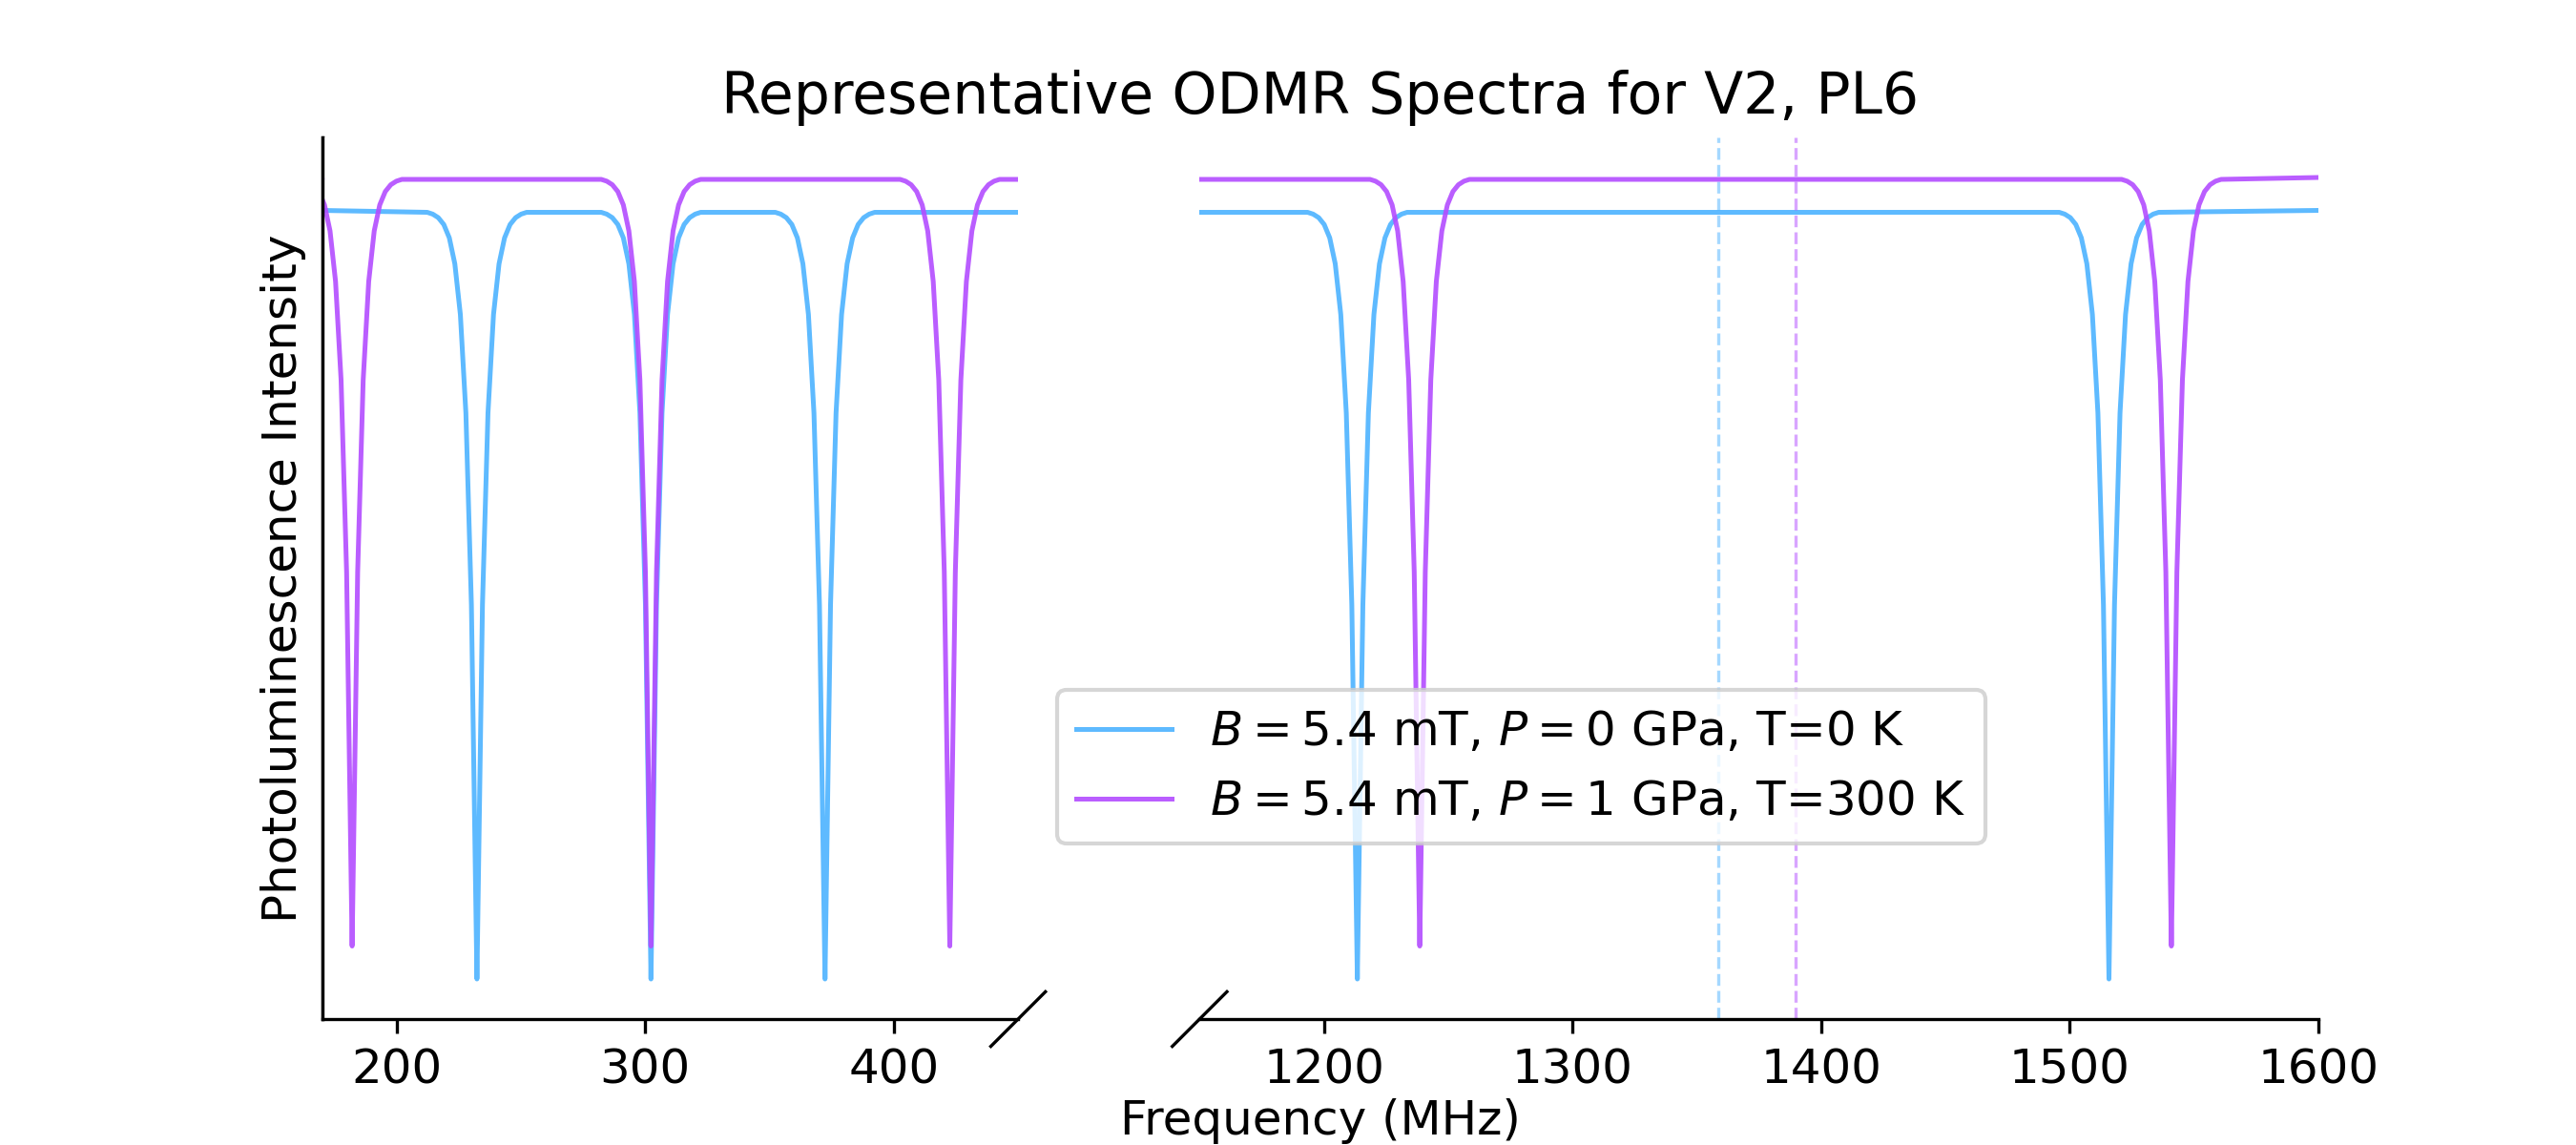
\includegraphics[width=0.95\textwidth]{figures/ODMR-multimodal-s15magnet-s1PT.png}
    \end{center}
    \caption{}\label{fig:multi-TP}
    \todo[inline, color=ediblue]{Write caption}
\end{figure}


% Theoretically, the measurement may be simultaneously completed using only the V2 Silicon vacancy, but temperature sensing using the 

% However, since for the V2 Silicon vacancy $D$ is not dependent on $T$ but linearly dependent on $P$, the pressure may be isolated by studying the spectra of that defect.

In practice, readily tuning lasers to respond to the effective $D$ may be impractical. If future work mapped a function $D(P,T)$ for the divacancy, it could be used to perform temperature measurement using only CW-ODMR techniques. 

To demonstrate, we (naively) assume the effects of temperature and pressure on the ZFS $D$ of the divacancy linearly combine, we visualise this in figure \ref{fig:multi-TP}. 

If all three frequencies are visible ($f_1 < f_2 < f_3$) in the $S=3/2$ spectra we see using \eqref{eq:spin1.5_magnet_Bparallel_eigenvalues} that we may determine $D$ using 
\begin{equation}
    D(P) = \frac{f_1 -f_3 }{4},
    \label{eq:}
\end{equation}
from which we infer the pressure $P_0$ as no dependence on $T$ is shown.     

We now fit the data to compute $T$ in the using the divacancy frequencies ($\nu_1, \nu_2$) as 
\begin{equation}
    D(T, P_0) = \frac{\nu_2 + \nu_1}{2}.
    \label{eq:}
\end{equation}
% this could be reduced by substitution of the measured pressure in the V2 defect ($P_0$), and a fit to the divacancy spectra of $D(P_0, T)$, from which we would determine $T$.

% \subsection{$\vec{E}$ Multimode}
\subsection{$\vec{E}$ and Temperature or Pressure}\label{multi-E-pressure}
The measurement of $\vec{E}$ in parallel to temperature (pressure) is less clear, as the influence of $E_\parallel$ is indistinguishable from a change in temperature (pressure) - a net change in ZFS $D$. Ideally, we would exploit the temperature independence of the V2 defect $D$ but we have been unable to find a schema for $S=3/2$ electrometry. 
Thus, within the context of this work we have been unable to find a scheme to simultaneously measure $\vec{E}$ and temperature (pressure) in general.  

An exception can be made however if careful alignment of the $\vec{E}$ is possible, then the magnitude may be measured. 

\begin{proposal}{$|\vec{E}|$ and Temperature (Pressure)}
    The $\vec{E}$ field is aligned perpendicular to the defect axis. Then by \eqref{eq:s1_elect_perp} we may determine the magnitude with no dependence on $D$. With knowledge of the $|\vec{E}|$, choose a defect on the same axis and calculate the influence of $\vec{E}$ on $D$ and $E$. Measure $D(\vec{E}, T)$ and fit the data to calculate the temperature (pressure) of the system. 
\end{proposal}

We infer from the electrometry Hamiltonian \eqref{eq:electometry_matrix_hamiltonian} that the corrections to $D$ and $E$ are 
\begin{equation}
    \Delta D = d_\parallel |\vec{E}| \cos\theta_E, \quad \Delta E = d_\perp |\vec{E}| \sin \theta_E.
    \label{eq:}
\end{equation}

We exploit that when $\theta = 90^\circ$ the ZFS $D$ is not affected by the field and any variation must be due to temperature (pressure). 

In the absence of an applied magnetic field (which would have to of known magnitude and applied parallel to the defect axis for this schema to work), $E$ is determined from the effective magnitude of ZFS $E$ by the difference in the frequencies as
\begin{equation}
    E_\perp d_\perp = E_0 - \sqrt{\frac{(f_1 - f_2)^2}{4} - (g \mu_B B)^2}, 
    \label{eq:multi-E+T}
\end{equation}
where $E_0$ is the ZFS $E$ of the defect without influence of the electric field. 

Temperature (pressure) sensing can also then be performed using the same two measured frequencies as $D(T)$ will be the average of them. 

Figure \ref{fig:E_Field_perp_temp} which shows a strictly perpendicular electric field allows a visualisation of the described effects.  
\begin{figure}[H]
    \begin{center}
        % 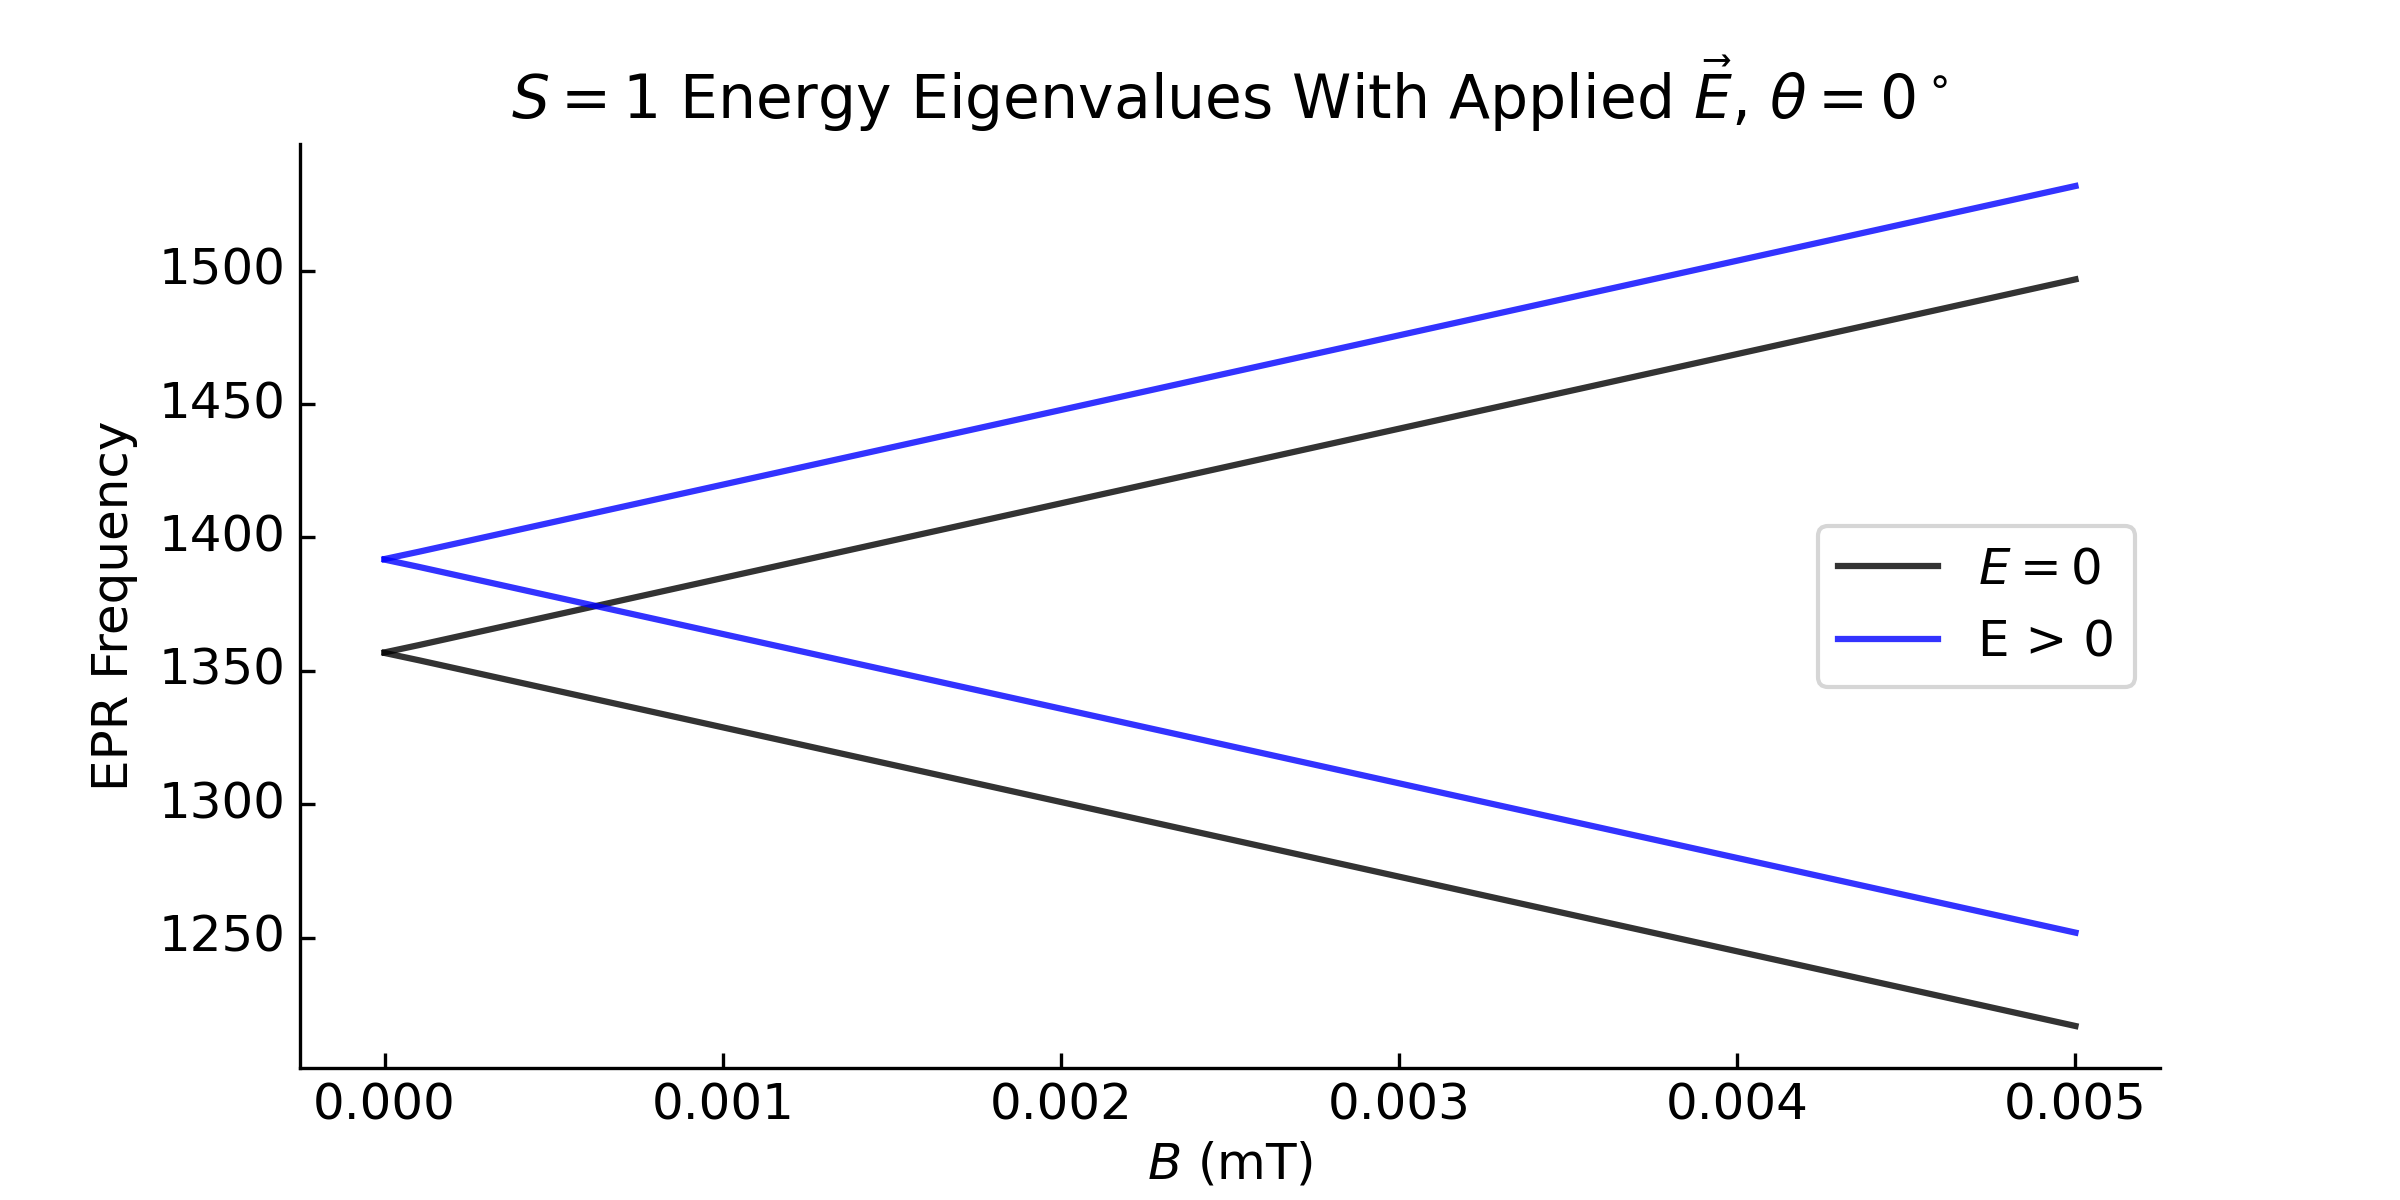
\includegraphics[width=0.95\textwidth]{figures/EFieldParallel.png}
        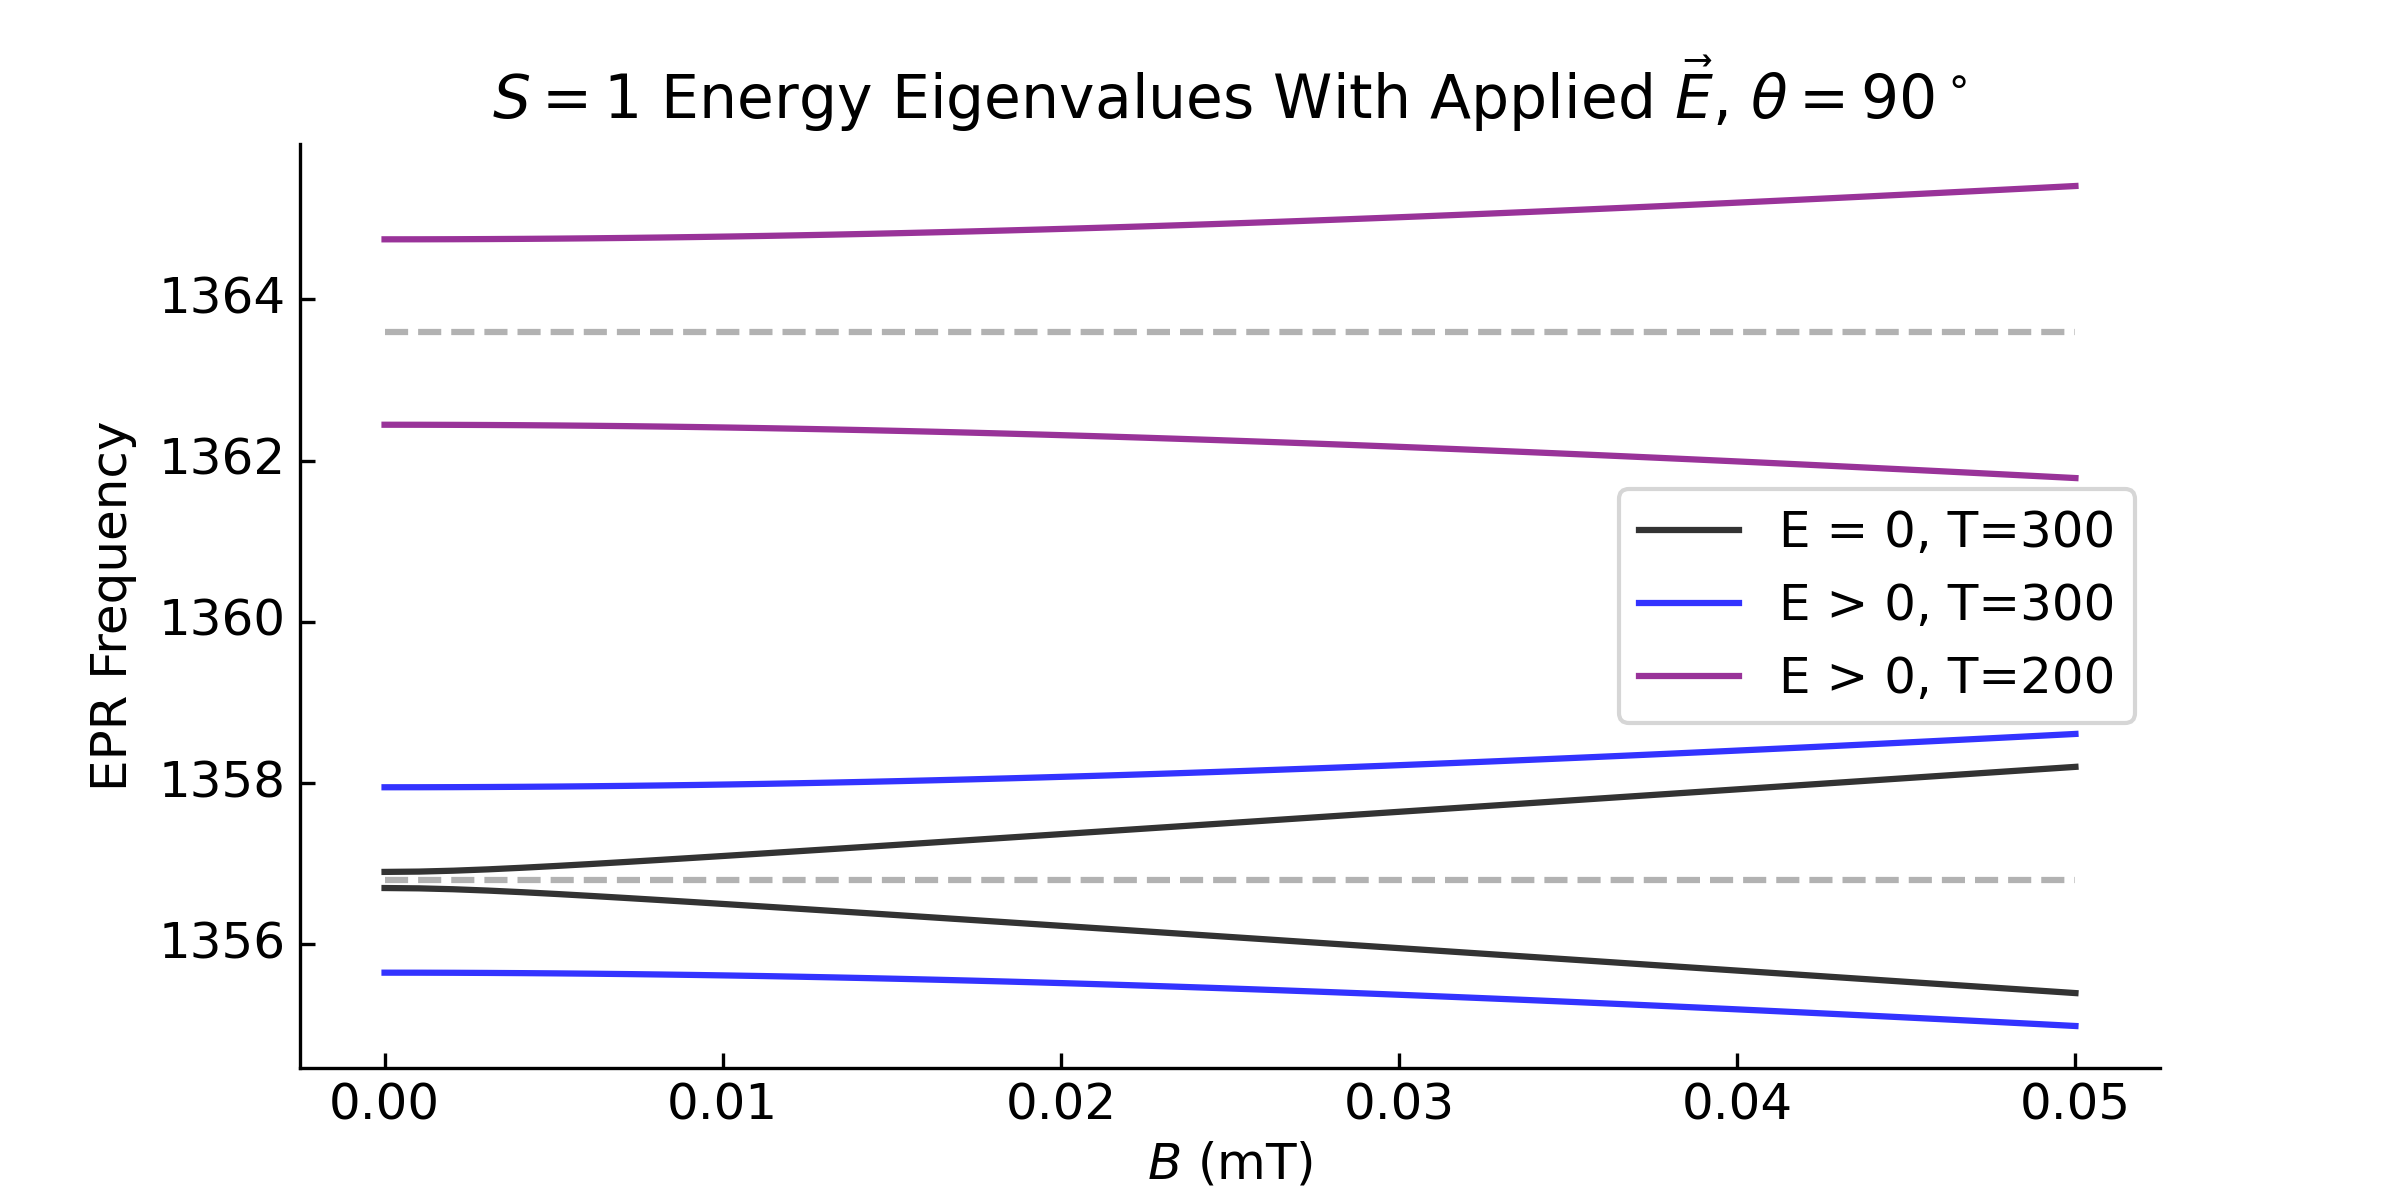
\includegraphics[width=0.95\textwidth]{figures/EFieldPerpTemp.png}
        % \missingfigure{ODMR/Energy plot showing effect of parallel/perp E field}
    \end{center}
    \caption{Eigenvalue plot showing... }\label{fig:E_Field_perp_temp}
    \todo[inline, color=ediblue]{Write caption}
\end{figure}

% \subsection{Scalar Sensing}

% Using a similar scheme to that described above...

\subsection{Trimodal $\vec{B}$, Temperature and Pressure}
% If we assume the interplay and dependence of temperature and pressure on the ZFS $D$ are well understood for the Silicon vacancy and the divacancy, then a trimodal schema is possible. 

\begin{proposal}{$\vec{B}$, Temperature and Pressure}
    We exploit the temperature independence of the V2 Silicon vacancy to perform a pressure measurement. Then, having fixed $P_0$, we infer $T$. Now, since $T$ and $P$ are well known, we may perform scalar magnetometry using either the $S=1$ or $S=3/2$ defects provided the magnetic field is aligned parallel to the defect axis. 
\end{proposal}

This method simply extends the method described in \ref{multi_TP}. By fixing the orientation of the field, the magnitude of the field may be computed from either the $S=1$ or $S=3/2$ spectra respectively as 
\begin{equation}
    B = \frac{\nu_2 - \nu_1}{2 g\mu_B }, \quad B = \frac{f_3 + f_1}{2 g \mu_B } = \frac{f_2}{g \mu_B}.  
    \label{eq:}
\end{equation}

% The only regime in which the magnitude of both fields may be simultaneously determined is identical to that described above in \ref{multi-E-pressure}. The discussion may be extended by measuring the magnitude of the magnetic field using \eqref{eq:s1_parallel_magnetometry} and substituting it into \eqref{eq:multi-E+T} to find 
% \begin{equation}
%     E_\perp d_\perp = E_0 - \sqrt{\frac{(f_1 - f_2)^2}{4} - (g \mu_B B)^2}, 
%     \label{eq:multi-E+T2}
% \end{equation}
%
%
% \subsection{Tri-modality}\label{sec:trimodal}
% The success of \ref{sec:multimode_BT} and possible encapsulation into a single defect type allowed for the consideration of a trimodal sensor.
%
% \begin{proposal}{$\vec{B}$, $\vec{E}$ and Temperature}
% 	The PL6 defect acts solely as a electrometer. We consider the influence of $\vec{B}$ and $T$ to be well known and extracted from V2 Silicon vacancy.
% \end{proposal}
%





% \subsection{$|\vec{B}|$ and $T$}
% \cite{Degen2008}
%
% \subsection{Angle Resolved $|\vec{B}|$ and $T$}
% % We show that uniaxial color centers in silicon carbide with hexagonal lattice structure can be used to measure not only the strength but also the polar angle of the external magnetic field with respect to the defect axis with high precision. 
% \cite{PhysRevApplied.4.014009}
%
% \subsection{$\vec{B}$ and $T$}
%
%
% \subsection{$|\vec{B}|$, $|\vec{E}|$ and $T$}
% The influence of an $\vec{E}$ field parallel to the defect axis is indistinguishable from the influence of a change of temperature. Similarly, the influence of an $\vec{E}$ field perpendicular to the defect axis is indistinguishable from the influence of a $\vec{B}$ field parallel to the defect axis. The exception is when \td{When $B_0$ is smaller than ZFS E when the effects can be distinguished}...
%
% \begin{figure}[H]
% 	\begin{center}
% 		% \includegraphics[width=0.95\textwidth]{figures/}
% 		\missingfigure{2 plots. Both of a basline energy graph and showing the similarity of T and parallel E, and B and perp E.}
% 	\end{center}
% 	\caption{\td{write caption}}\label{fig:}
% \end{figure}
%
%
% Thus, to extend the multi-modality to include the $\vec{E}$ field we must isolate the influence of the $\vec{E}$ field from the other environmental factors.
%
%
%
% \subsection{$\vec{B}$, $\vec{E}$ and $T$}
%
%
% % \begin{summary}{Multimodality Summary}{sum:multimodal}
% % 	From the construction of our multimodal systems we have learned
% % 	\begin{enumerate}
% % 		\item The Silicon vacancy is resistant to temperature fluctuations so can be used to measure $\vec{B}$ \textbf{or} $\vec{E}$ while a divacancy monitors temperature.
% % 	\end{enumerate}
% % \end{summary}
% %
%%%%%%%%%%%%%%%%%%%%%%%%%%%%%%%%%%%%%%%%%%%%%%%%%%%%%%%%%%%%%%%%%%%%%%%%%%%%%%%%%%%%%%%%%%%%%%%%%%%%%%%%%%%%%%%%%%%%%%%%%%%55

% \subsection{$\vec{B}$ and $\vec{E}$}
% Even more difficult is the separation of $\vec{B}$ and $\vec{E}$. 
% Using the techniques in this work no general solution was found for simultaneously measuring both fields.

